\documentclass[journal]{IEEEtran}

% ---- fonts -----------------------------------------------------------------
\usepackage{newtxtext}
\usepackage[vvarbb]{newtxmath}

% ---- maths -----------------------------------------------------------------
\usepackage{amsmath,amsfonts}

% ---- algorithms ------------------------------------------------------------
\usepackage{algorithm}
\usepackage{algpseudocode}

% ---- figures / tables ------------------------------------------------------
\usepackage{graphicx}
\graphicspath{{figs/}}
\usepackage{xcolor}
\usepackage{booktabs}
\usepackage{multirow}
\usepackage{array}
\usepackage{subfig}

% ---- typography ------------------------------------------------------------
\usepackage{textcomp}
\usepackage{microtype}

% ---- references / links ----------------------------------------------------
\usepackage{url}
\usepackage{cite}
\usepackage[hidelinks,
            pdftitle={SOM-TSK V3: A Unified Clustering Framework with Topology-Seeded Initialization, Density Discovery, and Automatic Pipeline Orchestration},
            pdfauthor={Evint Leovonzko}]{hyperref}

% ---- code listings ---------------------------------------------------------
\usepackage{listings}
\lstset{
  basicstyle=\ttfamily\footnotesize,
  columns=fullflexible,
  frame=single,
  breaklines=true,
  postbreak=\mbox{\textcolor{gray}{$\hookrightarrow$}\space},
}

% ---- misc ------------------------------------------------------------------
\usepackage{bm}

\DeclareMathOperator*{\argmin}{arg\,min}
\DeclareMathOperator*{\argmax}{arg\,max}

\urlstyle{same}
\raggedbottom

\begin{document}

\title{SOM-TSK V3: A Unified Clustering Framework with\\Topology-Seeded Initialization, Density Discovery,\\and Automatic Pipeline Orchestration}

\author{Evint Leovonzko%
\thanks{E. Leovonzko is with the Department of Computer Science and Engineering. Code: \protect\url{https://github.com/Evintkoo/SOM\_plus\_clustering}}}

\maketitle

\begin{abstract}
We present \textit{SOM-TSK~V3}, a unified clustering framework combining topology-seeded $K$-means (SOM-TSK), density-based SOM clustering (DenSOM), Gaussian Mixture Models (GMM), and automatic algorithm selection (AutoSOM) under a plugin-based pipeline architecture.
V3 extends the prior SOM-TSK framework---which on this V3 multi-seed benchmark achieves 3~wins, 19~ties, and 2~losses against KMeans++ across 24~datasets (statistically equivalent on average; Wilcoxon $p = 0.765$)---with three contributions:
(i)~a \texttt{ClusteringPipeline} supporting runtime algorithm registration and Hopkins-statistic fast-path routing;
(ii)~diagonal-covariance GMM with BIC model selection as a first-class algorithm;
(iii)~a systematic UMAP preprocessing study showing that manifold embedding \emph{degrades} SOM-TSK on low-dimensional data (mean $\Delta\mathrm{ARI} = -0.10$).
Effect-size analysis (Cohen's $d$, Cliff's $\delta$, $B{=}5000$ bootstrap resamples) confirms that the Digits win represents a very large practical effect ($d = 8.85$), while the remaining differences are small or within sampling noise.
We additionally provide per-phase profiling, memory characterization, a failure-mode taxonomy, and a practitioner decision framework.
The implementation is in safe Rust with optional CUDA/Metal GPU backends and trains in under 10\,s for $n \le 50{,}000$.
\end{abstract}

\begin{IEEEkeywords}
Self-Organizing Map, clustering pipeline, topology-seeded initialization, density-based clustering, Gaussian mixture model, UMAP, effect size, practical guidelines
\end{IEEEkeywords}


\section{Introduction}
\label{sec:introduction}

\IEEEPARstart{C}{lustering} remains one of the most widely studied problems in unsupervised machine learning. The $K$-means algorithm~\cite{macqueen1967some,lloyd1982least} dominates practical applications owing to its simplicity and scalability, yet its quality is notoriously initialization-sensitive: random centroid placement routinely traps the algorithm in suboptimal local minima~\cite{arthur2007kmeans}. The KMeans++ initialization strategy~\cite{arthur2007kmeans} mitigates this by spreading seeds proportional to squared distance, achieving an $\mathcal{O}(\log k)$ approximation guarantee in expectation. Nevertheless, a single KMeans++ draw can still produce a poor partition when clusters are highly overlapping, imbalanced, or when $k$ is large relative to dataset size.

Self-Organizing Maps (SOMs)~\cite{kohonen1982self,kohonen2001self} offer a complementary view of the data: by learning a low-dimensional neuron grid that approximates the data manifold, a trained SOM implicitly encodes global topology---neighbourhood relationships, density variation, and inter-cluster structure---in its weight matrix. This information is not exploited by standard KMeans initialization.

The V2 paper~\cite{somtskv2} reported SOM-TSK as a reliable improvement over KMeans++, achieving 6 wins, 18 ties, and 0 losses across 24 benchmark datasets under a single-seed KMeans++ baseline. Under the stricter V3 multi-seed protocol (10 KMeans++ restarts, best inertia retained), this margin narrows to 3 wins, 19 ties, and 2 losses, with no statistically significant pairwise difference---a finding we report transparently below. However, V2 left several practical questions unanswered: (i) How should practitioners choose between SOM-TSK, DenSOM, GMM, and KMeans++ for a given dataset? (ii) What is the computational breakdown across pipeline phases? (iii) Does UMAP preprocessing---increasingly popular in practice---complement or conflict with SOM-based initialization? (iv) How large are the observed improvements in practical terms (effect sizes)?

\textbf{Contributions.} This paper makes the following contributions beyond V2:

\begin{enumerate}
\item \textbf{Unified Pipeline Architecture.} We formalize the \texttt{ClusteringPipeline}---a plugin-based orchestration layer that registers algorithms at runtime, routes datasets via Hopkins-statistic fast-path detection, and provides progress callbacks for interactive use. This enables practitioners to swap algorithms without code changes.

\item \textbf{GMM as First-Class Algorithm.} We integrate diagonal-covariance Gaussian Mixture Models with EM fitting and BIC model selection as a standalone clustering option, completing the algorithm suite for datasets with overlapping Gaussian structure.

\item \textbf{UMAP Preprocessing Analysis.} We conduct a systematic evaluation of UMAP dimensionality reduction as a preprocessing step, revealing that it \emph{degrades} SOM-TSK on low-dimensional data (mean $\Delta$ARI $= -0.12$ on 2D datasets) while providing inconsistent gains on high-dimensional data.

\item \textbf{Extended Practical Analysis.} We provide per-phase computational profiling, memory footprint characterization, a failure-mode taxonomy with decision guidelines, and effect-size analysis using Cohen's $d$ and Cliff's delta.

\item \textbf{Practitioner Decision Framework.} We synthesize all findings into an actionable decision tree for algorithm selection based on dataset characteristics ($n$, $d$, $k$, cluster geometry, time budget).
\end{enumerate}

\section{Related Work}
\label{sec:related}

\subsection{$K$-means Initialization}

The sensitivity of $K$-means to initialization has motivated extensive research. Arthur and Vassilvitskii~\cite{arthur2007kmeans} proved that KMeans++ achieves an $\mathcal{O}(\log k)$ competitive ratio in expectation. Bahmani et al.~\cite{bahmani2012scalable} proposed $k$-means$\|$, a scalable parallel initialization. Celebi et al.~\cite{celebi2013comparative} conducted a comprehensive comparison of thirteen initialization methods, finding that careful deterministic strategies often outperform random ones. Katsavounidis et al.~\cite{katsavounidis1994new} proposed a max-distance greedy seeding similar to our SOM++ initialization.

\subsection{SOM-Based Clustering}

Kohonen~\cite{kohonen2013essentials} provided an updated account of the SOM's properties as a topology-preserving manifold approximator. Vesanto and Alhoniemi~\cite{vesanto2000clustering} extended this by comparing KMeans with Ward linkage for neuron-level post-processing. Ta\c{s}demir and Merenyi~\cite{tasdemir2009exploiting} showed that the SOM's implicit data adjacency topology can reveal cluster boundaries invisible to standard metrics.

\subsection{Dimensionality Reduction for Clustering}

UMAP~\cite{mcinnes2018umap} has become the de facto standard for visualization and preprocessing in high-dimensional clustering workflows. Several studies~\cite{allaoui2020considerably,kobak2021initialization} have shown that UMAP followed by KMeans or HDBSCAN can improve clustering on high-dimensional data. However, the interaction between UMAP and SOM-based methods has not been studied. We address this gap with a systematic comparison.

\subsection{Gaussian Mixture Models}

GMMs~\cite{fraley2002model,mclachlan2019finite} provide a probabilistic framework for clustering that naturally handles overlapping clusters and provides uncertainty estimates. BIC-based model selection~\cite{schwarz1978estimating} offers principled $k$-estimation. Our integration of GMM into the SOM-TSK pipeline provides a complementary algorithm for datasets where Gaussian assumptions hold.

\subsection{Clustering Pipelines and AutoML}

The AutoML movement~\cite{hutter2019automated} has produced systems like Auto-sklearn~\cite{feurer2015efficient} and CASH~\cite{thornton2013auto} that automate algorithm selection. Our \texttt{ClusteringPipeline} takes a more focused approach: rather than searching over all possible algorithms, it uses data-driven heuristics (Hopkins statistic, BIC) to route to the most appropriate algorithm from a curated set.

\subsection{Effect Size in Machine Learning Evaluation}

Recent work~\cite{demsar2006statistical,benavoli2017time} has emphasized that statistical significance alone is insufficient for evaluating ML algorithms---practical effect size matters. We adopt Cohen's $d$~\cite{cohen1988statistical} and Cliff's delta~\cite{cliff1993dominance} to quantify the magnitude of SOM-TSK's improvements, complementing the bootstrap significance tests from V2.


\section{Background}
\label{sec:background}

\subsection{Self-Organizing Maps}

A Self-Organizing Map places $M = m \times n$ prototype neurons $\{\mathbf{w}_j \in \mathbb{R}^d\}_{j=1}^{M}$ on a 2D rectangular grid. Training updates each neuron by the competitive learning rule:
\begin{equation}
  \mathbf{w}_j(t+1) = \mathbf{w}_j(t) + \alpha(t)\,h_{c,j}(t)\bigl[\mathbf{x}(t) - \mathbf{w}_j(t)\bigr],
  \label{eq:som_update}
\end{equation}
where $c = \argmin_j \|\mathbf{x}(t) - \mathbf{w}_j\|$ is the Best-Matching Unit (BMU), $\alpha(t)$ is the learning rate, and $h_{c,j}(t) = \exp\!\bigl(-\|r_c - r_j\|^2/(2\sigma^2(t))\bigr)$ is the Gaussian neighbourhood kernel. Both $\alpha$ and $\sigma$ decay linearly over $T$ epochs.

\subsection{KMeans and KMeans++}

$K$-means minimizes inertia $\mathcal{I} = \sum_{i=1}^n \|\mathbf{x}_i - \boldsymbol{\mu}_{c_i}\|^2$ by alternating label assignment and centroid update. KMeans++~\cite{arthur2007kmeans} seeds centroids by sampling proportional to $D(\mathbf{x})^2$.

\subsection{Gaussian Mixture Models}

A $k$-component diagonal-covariance GMM models data as:
\begin{equation}
  p(\mathbf{x}) = \sum_{c=1}^k \pi_c \prod_{j=1}^d \mathcal{N}(x_j \mid \mu_{c,j}, \sigma^2_{c,j}),
\end{equation}
where $\pi_c$ are mixing weights. The EM algorithm alternates between computing responsibilities (E-step) and updating parameters (M-step). Model selection uses BIC:
\begin{equation}
  \mathrm{BIC}(k) = -2\ell_k + p_k \ln n, \quad p_k = k(2d+1) - 1.
\end{equation}

\subsection{Hopkins Statistic}

The Hopkins statistic~\cite{hopkins1954new} measures clustering tendency by comparing nearest-neighbour distances in the data to those from a uniform reference:
\begin{equation}
  H = \frac{\sum_{i=1}^m u_i}{\sum_{i=1}^m u_i + \sum_{i=1}^m w_i},
\end{equation}
where $u_i$ are nearest-neighbour distances from uniform random points to data, and $w_i$ are nearest-neighbour distances within a data subsample. $H > 0.5$ indicates clustering tendency; $H > 0.85$ indicates well-separated clusters.

\subsection{UMAP}

Uniform Manifold Approximation and Projection~\cite{mcinnes2018umap} constructs a fuzzy topological representation of high-dimensional data and optimizes a low-dimensional embedding that preserves this structure. Key parameters are $n_{\text{neighbors}}$ (local connectivity) and $\min\_dist$ (embedding compactness).

\section{The SOM-TSK Framework (Review)}
\label{sec:som_tsk}

We briefly review the SOM-TSK pipeline from V2 for completeness. The full pipeline consists of:

\begin{enumerate}
\item \textbf{SOM Training} with SOM++ initialization (deterministic farthest-point sampling).
\item \textbf{Phase A}: KMeans++ on the neuron grid, mapped to data-space centroids.
\item \textbf{Phase A-alt}: Maximum-spread neuron seeding via greedy farthest-point.
\item \textbf{Phase B-bis}: Multi-start coverage-aware density seeding from top-3 hit-count neurons.
\item \textbf{Phase C}: Fresh KMeans++ on raw data (deterministic baseline).
\item \textbf{Selection}: Inertia-windowed ($\rho = 1.05$) Calinski--Harabasz maximization.
\end{enumerate}

The selection criterion is:
\begin{equation}
  \hat{\mathbf{y}} = \argmax_{\mathbf{y} \in \mathcal{P}_{1.05}} \mathrm{CH}(\mathbf{y}), \quad \mathcal{P}_\rho = \{\mathbf{y} : \mathcal{I}(\mathbf{y}) \le \rho \cdot \mathcal{I}^*\}.
\end{equation}

\section{V3 Additions: Unified Pipeline and GMM}
\label{sec:v3_additions}

\subsection{The ClusteringPipeline Architecture}

V3 introduces a unified \texttt{ClusteringPipeline} that orchestrates all algorithms through a common interface. The architecture consists of three layers:

\textbf{Layer 1: Plugin Registry.} A runtime registry maps algorithm names to factory closures. Each \texttt{get(name)} call returns a fresh, unfitted instance, enabling stateless parallel evaluation. The registry validates names (1--128 ASCII characters) and prevents duplicate registration.

\textbf{Layer 2: Algorithm Trait.} All algorithms implement a common \texttt{ClusteringAlgorithm} trait with three methods:
\begin{itemize}
  \item \texttt{fit(data)} --- Train the model on data.
  \item \texttt{predict(data)} --- Assign cluster labels.
  \item \texttt{fit\_predict(data)} --- Convenience: fit then predict.
\end{itemize}

\textbf{Layer 3: Pipeline Orchestration.} The pipeline provides:
\begin{itemize}
  \item \texttt{run(algorithm, data)} --- Execute a named algorithm.
  \item \texttt{run\_auto(data)} --- Automatic algorithm selection via Hopkins statistic.
  \item \texttt{with\_progress\_callback(f)} --- Progress reporting for interactive use.
  \item Automatic metric computation (silhouette, noise ratio) on results.
\end{itemize}

\begin{algorithm}
\caption{ClusteringPipeline.run\_auto}
\label{alg:pipeline_auto}
\begin{algorithmic}[1]
\Require Data $\mathbf{X} \in \mathbb{R}^{n \times d}$, config $\mathcal{C}$
\Ensure  \texttt{PipelineResult} with labels, metrics, algorithm name
\State $H \leftarrow \text{Hopkins}(\mathbf{X})$ \Comment{Clustering tendency}
\If{$\mathcal{C}.\text{fast\_path\_enabled}$ \textbf{and} $H > \mathcal{C}.\text{threshold}$}
  \State \Return \texttt{run("kmeans", $\mathbf{X}$)} with \texttt{fast\_path = true}
\Else
  \State \Return \texttt{run("autosom", $\mathbf{X}$)}
\EndIf
\end{algorithmic}
\end{algorithm}

The Hopkins-based fast-path (Algorithm~\ref{alg:pipeline_auto}) avoids the full SOM training overhead on datasets where KMeans++ already achieves optimal results. With threshold $H > 0.85$, this correctly identifies well-separated Gaussian blobs (scale\_*, dim\_*) and routes them directly to KMeans, saving 200--800$\times$ computation.

\subsection{GMM as First-Class Algorithm}

V3 elevates GMM from an internal component of AutoSOM's $k$-selection to a standalone clustering algorithm. The implementation features:

\begin{itemize}
  \item \textbf{Diagonal covariance}: $\mathcal{O}(nkd)$ per EM iteration (vs.\ $\mathcal{O}(nkd^2)$ for full covariance), enabling scaling to $d=256$.
  \item \textbf{Multi-restart}: $R=3$ independent EM runs with deterministic seeding; best log-likelihood retained.
  \item \textbf{KMeans++ warm start}: Initial means from KMeans++; initial variances from within-cluster variance; initial weights uniform.
  \item \textbf{Variance floor}: $\sigma^2_{c,j} \ge 10^{-6}$ prevents degenerate components.
  \item \textbf{BIC model selection}: Sweep $k \in \{2, \ldots, k_{\max}\}$ and select $\hat{k} = \argmin_k \mathrm{BIC}(k)$.
\end{itemize}

The GMM wrapper implements the \texttt{ClusteringAlgorithm} trait, making it interchangeable with KMeans, DenSOM, and AutoSOM in the pipeline.

\subsection{Registered Algorithms}

The built-in pipeline registers four algorithms:

\begin{table}[!t]
\caption{Built-in Pipeline Algorithms}
\label{tab:algorithms}
\centering
\renewcommand{\arraystretch}{1.1}
\small
\begin{tabular}{llll}
\toprule
Name & Type & $k$ Required & Noise Support \\
\midrule
\texttt{kmeans} & Centroid-based & Yes & No \\
\texttt{gmm} & Model-based & Yes & No \\
\texttt{densom} & Density-based & No (auto) & Yes \\
\texttt{autosom} & Meta-algorithm & No (auto) & Yes \\
\bottomrule
\end{tabular}
\end{table}

Custom algorithms can be registered at runtime via \texttt{register\_algorithm(name, factory)}, enabling domain-specific extensions without modifying the core library.


\section{UMAP Preprocessing Analysis}
\label{sec:umap}

A common modern workflow applies UMAP dimensionality reduction before clustering. We systematically evaluate whether UMAP preprocessing benefits or harms SOM-TSK and KMeans++ across all 24 benchmark datasets.

\subsection{Experimental Setup}

UMAP is applied with $n_{\text{neighbors}} = 15$, $\min\_dist = 0.1$, target dimension $d' = \min(d, 10)$ for $d > 10$ and $d' = d$ otherwise (i.e., no reduction for already-low-dimensional data, but the UMAP graph structure still transforms the embedding). Both SOM-TSK and KMeans++ are then run on the UMAP-transformed data with the same hyperparameters as the baseline experiments.

\subsection{Results}

\begin{table}[!t]
\caption{UMAP Preprocessing Impact: $\Delta$ARI = UMAP $-$ Baseline}
\label{tab:umap}
\centering
\renewcommand{\arraystretch}{1.05}
\small
\setlength{\tabcolsep}{3pt}
\begin{tabular}{lcccc}
\toprule
\multirow{2}{*}{Category} & \multicolumn{2}{c}{SOM-TSK} & \multicolumn{2}{c}{KMeans++} \\
\cmidrule(lr){2-3}\cmidrule(lr){4-5}
 & Mean $\Delta$ARI & Wins/Losses & Mean $\Delta$ARI & Wins/Losses \\
\midrule
S-sets (2D, $k$=15) & $-0.175$ & 0/4 & $-0.003$ & 0/1 \\
A-sets (2D, $k$=20--50) & $-0.268$ & 0/3 & $-0.048$ & 0/2 \\
Shapes (2D) & $-0.044$ & 1/2 & $+0.012$ & 1/1 \\
UCI ($d$=4--64) & $-0.032$ & 1/2 & $+0.019$ & 2/1 \\
Scalability (2D) & $-0.001$ & 0/0 & $-0.001$ & 0/0 \\
High-dim ($d$=32--256) & $+0.000$ & 0/0 & $+0.000$ & 0/0 \\
\midrule
\textbf{Overall} & $\mathbf{-0.097}$ & 2/11 & $\mathbf{-0.006}$ & 3/5 \\
\bottomrule
\end{tabular}
\end{table}

\subsection{Key Findings}

\textbf{Finding 1: UMAP degrades SOM-TSK on low-dimensional data.} On the 2D SIPU datasets (S-sets, A-sets), UMAP preprocessing causes catastrophic degradation of SOM-TSK (mean $\Delta$ARI $= -0.22$). The SOM's topology-preserving properties are disrupted by UMAP's nonlinear distortion of the already-interpretable 2D geometry. The SOM trains on UMAP-distorted coordinates, producing a neuron grid that no longer reflects the true cluster structure.

\textbf{Finding 2: KMeans++ is more robust to UMAP.} KMeans++ shows smaller degradation (mean $\Delta$ARI $= -0.006$) because it does not rely on manifold structure---it only needs well-separated centroids, which UMAP generally preserves.

\textbf{Finding 3: UMAP provides no benefit on already-separated data.} On the scalability and high-dimensional benchmarks (where clusters are well-separated Gaussians), UMAP adds computation without improving ARI for either algorithm.

\textbf{Finding 4: UMAP may help on specific high-$d$ non-Gaussian datasets.} On Digits ($d=64$), UMAP+KMeans++ achieves ARI $= 0.62$ vs.\ baseline KMeans++ ARI $= 0.35$, a substantial improvement. However, SOM-TSK \emph{without} UMAP already achieves ARI $= 0.58$, suggesting that the SOM's manifold learning provides similar benefits to UMAP for this dataset class.

\subsection{Practical Recommendation}

\begin{quote}
\textit{Do not apply UMAP before SOM-TSK.} The SOM already performs manifold learning; adding UMAP creates a redundant and potentially harmful double-embedding. For KMeans++ on high-dimensional non-Gaussian data, UMAP preprocessing can be beneficial, but SOM-TSK without UMAP often achieves comparable results.
\end{quote}

\section{Experimental Setup}
\label{sec:experiments}

\subsection{Datasets}

We evaluate on the same 24 datasets from V2, spanning five categories: SIPU S-sets ($k=15$, $n=4995$), SIPU A-sets ($k=20$--$50$), synthetic shapes, UCI real-world (Iris, Wine, Breast Cancer, Digits), scalability ($n=1000$--$50000$), and high-dimensional ($d=32$--$256$). Full details are in Table~\ref{tab:datasets}.

\begin{table}[!t]
\caption{Benchmark Dataset Summary}
\label{tab:datasets}
\centering
\renewcommand{\arraystretch}{1.05}
\small
\begin{tabular}{lrrrrl}
\toprule
Dataset & $n$ & $d$ & $k$ & SOM Grid & Difficulty \\
\midrule
\multicolumn{6}{l}{\textit{SIPU S-sets (increasing overlap)}} \\
s1 & 4,995 & 2 & 15 & $8{\times}8$ & Easy \\
s2 & 4,995 & 2 & 15 & $8{\times}8$ & Medium \\
s3 & 4,995 & 2 & 15 & $8{\times}8$ & Hard \\
s4 & 4,995 & 2 & 15 & $8{\times}8$ & Very Hard \\
\multicolumn{6}{l}{\textit{SIPU A-sets (increasing $k$)}} \\
a1 & 3,000 & 2 & 20 & $9{\times}9$ & Medium \\
a2 & 5,250 & 2 & 35 & $12{\times}12$ & Hard \\
a3 & 7,500 & 2 & 50 & $15{\times}15$ & Very Hard \\
\multicolumn{6}{l}{\textit{Synthetic shapes (non-convex)}} \\
moons & 300 & 2 & 2 & $5{\times}5$ & KMeans-hard \\
circles & 300 & 2 & 2 & $5{\times}5$ & KMeans-hard \\
spiral & 300 & 2 & 3 & $5{\times}5$ & KMeans-hard \\
anisotropic & 300 & 2 & 3 & $5{\times}5$ & Easy \\
varied\_density & 1,000 & 2 & 3 & $5{\times}5$ & Medium \\
\multicolumn{6}{l}{\textit{UCI real-world}} \\
Iris & 150 & 4 & 3 & $5{\times}5$ & Easy \\
Wine & 178 & 13 & 3 & $5{\times}5$ & Medium \\
Breast Cancer & 569 & 30 & 2 & $6{\times}6$ & Medium \\
Digits & 500 & 64 & 10 & $8{\times}8$ & Hard \\
\multicolumn{6}{l}{\textit{Scalability ($d=2$, $k=5$, well-separated)}} \\
scale\_1k--50k & 1k--50k & 2 & 5 & $10{\times}10$ & Easy \\
\multicolumn{6}{l}{\textit{High-dimensional ($n=1000$, $k=5$, well-separated)}} \\
dim\_32--256 & 1,000 & 32--256 & 5 & $8{\times}8$ & Easy \\
\bottomrule
\end{tabular}
\end{table}

\subsection{Evaluation Metrics}

We report six metrics: ARI, NMI, FMI (external, require ground truth), Silhouette, Davies--Bouldin, Calinski--Harabasz (internal, no ground truth needed). Win/tie/loss threshold: $|\Delta\mathrm{ARI}| > 0.005$.

\subsection{Effect Size Measures}

Beyond statistical significance, we report:
\begin{itemize}
  \item \textbf{Cohen's $d$}: Standardized mean difference of bootstrap $\Delta$ARI distributions. $|d| > 0.8$ = large effect.
  \item \textbf{Cliff's $\delta$}: Non-parametric effect size measuring the probability that a random SOM-TSK resample outperforms a random KMeans++ resample. $|\delta| > 0.474$ = large effect.
\end{itemize}

\subsection{Implementation and Environment}

All algorithms are implemented in safe Rust (edition 2021). Key dependencies: \texttt{ndarray} 0.16 (with Rayon parallelism), \texttt{rand} 0.9. Optional CUDA (\texttt{cudarc} 0.12) and Metal (\texttt{metal} 0.33) backends via feature flags. Release profile: \texttt{opt-level=3}, \texttt{lto="fat"}, \texttt{codegen-units=1}.

\textbf{Hardware.} Apple M2 Pro (12-core CPU, 19-core GPU), 16\,GB unified memory, macOS~14 Sonoma (arm64). All timings are wall-clock, single-process, averaged over 5~runs.

\textbf{Baselines.} KMeans++ uses the same Rust implementation with 10~independent restarts (best inertia retained). SOM-TSK is fully deterministic (single run, no RNG). GMM uses 3~EM restarts with KMeans++ warm-start.

\textbf{Reproducibility.} All experiments are reproducible via the benchmark scripts in the repository. No randomness enters SOM-TSK; KMeans++ baselines use a fixed seed sequence $\{42, 43, \ldots, 51\}$.


\section{Results}
\label{sec:results}

\subsection{Main Results: SOM-TSK vs.\ KMeans++ (Verified Identical to V2)}

Table~\ref{tab:main_results} updates the V2 findings with the V3 multi-seed benchmark: SOM-TSK achieves \textbf{3 wins, 19 ties, 2 losses} against KMeans++ across all 24 datasets. Mean ARI improvement: $+0.0076$. The three wins span high-$k$ (s3), high-$d$ (Digits), and moderate-$d$ (Wine) datasets; the two losses (Iris, Breast Cancer) are small ($|\Delta\text{ARI}| \le 0.025$).

\textbf{V2$\to$V3 clustering quality.} The SOM-TSK algorithm is unchanged between V2 and V3; all 24 ARI values are bit-for-bit identical. V3's contributions are architectural (pipeline, trait system), algorithmic breadth (GMM, AutoSOM as alternatives), performance (optimized math, Metal GPU), and analytical (UMAP study, effect sizes, statistical tests). The core SOM-TSK seeding phases and selection criterion remain the same.

\begin{table*}[!t]
\caption{Main Results: ARI, NMI, FMI for SOM-TSK vs.\ KMeans++ across all 24 benchmark datasets. $\Delta$ARI $= \text{SOM-TSK} - \text{KMeans++}$; W/T/L threshold $= 0.005$.}
\label{tab:main_results}
\centering
\renewcommand{\arraystretch}{1.05}
\setlength{\tabcolsep}{4pt}
\begin{tabular}{lcccccccc}
\toprule
\multirow{2}{*}{Dataset} & \multicolumn{3}{c}{SOM-TSK} & \multicolumn{3}{c}{KMeans++} & \multirow{2}{*}{$\Delta$ARI} & \multirow{2}{*}{Result} \\
\cmidrule(lr){2-4}\cmidrule(lr){5-7}
 & ARI & NMI & FMI & ARI & NMI & FMI & & \\
\midrule
s1 & 0.976 & 0.976 & 0.978 & 0.976 & 0.976 & 0.978 & $+0.000$ & Tie \\
s2 & 0.579 & 0.735 & 0.607 & 0.578 & 0.735 & 0.607 & $+0.001$ & Tie \\
s3 & \textbf{0.319} & \textbf{0.530} & \textbf{0.364} & 0.311 & 0.528 & 0.357 & $\mathbf{+0.008}$ & \textbf{Win} \\
s4 & 0.186 & 0.397 & 0.244 & 0.189 & 0.397 & 0.244 & $-0.003$ & Tie \\
a1 & 0.977 & 0.980 & 0.978 & 0.977 & 0.980 & 0.978 & $+0.000$ & Tie \\
a2 & 0.800 & 0.882 & 0.806 & 0.800 & 0.882 & 0.806 & $+0.000$ & Tie \\
a3 & 0.583 & 0.792 & 0.591 & 0.579 & 0.791 & 0.588 & $+0.004$ & Tie \\
moons & 0.479 & 0.382 & 0.739 & 0.479 & 0.382 & 0.739 & $+0.000$ & Tie \\
circles & $-0.003$ & 0.000 & 0.497 & $-0.003$ & 0.000 & 0.497 & $+0.000$ & Tie \\
spiral & 0.016 & 0.026 & 0.349 & 0.018 & 0.023 & 0.345 & $-0.002$ & Tie \\
anisotropic & 1.000 & 1.000 & 1.000 & 1.000 & 1.000 & 1.000 & $+0.000$ & Tie \\
varied\_density & 0.446 & 0.557 & 0.669 & 0.445 & 0.557 & 0.669 & $+0.000$ & Tie \\
Iris & 0.620 & 0.673 & 0.759 & 0.645 & 0.661 & 0.762 & $-0.025$ & Loss \\
Wine & \textbf{0.898} & \textbf{0.876} & \textbf{0.932} & 0.880 & 0.861 & 0.921 & $\mathbf{+0.017}$ & \textbf{Win} \\
Breast Cancer & 0.654 & 0.562 & 0.853 & 0.677 & 0.562 & 0.853 & $-0.023$ & Loss \\
Digits & \textbf{0.554} & \textbf{0.742} & \textbf{0.627} & 0.349 & 0.540 & 0.462 & $\mathbf{+0.205}$ & \textbf{Win} \\
\multicolumn{9}{l}{\textit{Scalability ($d=2$, $k=5$, well-separated)}} \\
scale\_1k & 0.980 & 0.978 & 0.982 & 0.980 & 0.978 & 0.982 & $+0.000$ & Tie \\
scale\_5k & 0.981 & 0.979 & 0.983 & 0.981 & 0.979 & 0.983 & $+0.000$ & Tie \\
scale\_10k & 0.982 & 0.980 & 0.984 & 0.982 & 0.980 & 0.984 & $+0.000$ & Tie \\
scale\_25k & 0.983 & 0.981 & 0.985 & 0.983 & 0.981 & 0.985 & $+0.000$ & Tie \\
scale\_50k & 0.984 & 0.982 & 0.986 & 0.984 & 0.982 & 0.986 & $+0.000$ & Tie \\
\multicolumn{9}{l}{\textit{High-dimensional ($n=1000$, $k=5$, well-separated)}} \\
dim\_32 & 1.000 & 1.000 & 1.000 & 1.000 & 1.000 & 1.000 & $+0.000$ & Tie \\
dim\_64 & 1.000 & 1.000 & 1.000 & 1.000 & 1.000 & 1.000 & $+0.000$ & Tie \\
dim\_128 & 1.000 & 1.000 & 1.000 & 1.000 & 1.000 & 1.000 & $+0.000$ & Tie \\
dim\_256 & 1.000 & 1.000 & 1.000 & 1.000 & 1.000 & 1.000 & $+0.000$ & Tie \\
\midrule
\textbf{Mean} & \textbf{0.709} & \textbf{0.748} & \textbf{0.787} & 0.701 & 0.741 & 0.781 & $+0.008$ & 3W/19T/2L \\
\bottomrule
\end{tabular}
\end{table*}

\subsection{Effect Size Analysis}
\label{sec:effect_size}

\begin{figure}[!t]
\centering

\includegraphics[width=\columnwidth]{figs/delta_ari.pdf}
\caption{ARI gain ($\Delta$ARI = SOM-TSK $-$ KMeans++) per dataset. Blue lollipops indicate wins ($\Delta > 0.005$); gray indicates ties; red indicates the two small losses (Iris, Breast Cancer).}
\label{fig:delta_ari}
\end{figure}

Table~\ref{tab:effect_size} reports effect sizes for the three winning datasets, computed from $B=5000$ bootstrap resamples.

\begin{table}[!t]
\caption{Effect Size Analysis for SOM-TSK Wins ($B=5000$ bootstrap resamples)}
\label{tab:effect_size}
\centering
\renewcommand{\arraystretch}{1.1}
\small
\setlength{\tabcolsep}{3pt}
\begin{tabular}{lcccccl}
\toprule
Dataset & $\Delta$ARI & 95\% CI & $\hat{p}$ & Cohen's $d$ & Cliff's $\delta$ & Magnitude \\
\midrule
s3 & $+0.008$ & $[-.000,+.016]$ & 0.97 & 1.83 & 0.95 & Large \\
Wine & $+0.017$ & $[-.035,+.079]$ & 0.61 & 0.30 & 0.22 & Small \\
Digits & $+0.205$ & $[+.155,+.258]$ & 1.00 & 8.85 & 1.00 & Large \\
\bottomrule
\end{tabular}
\end{table}

\textbf{Interpretation.} The Digits win exhibits a \emph{very large} effect size: Cohen's $d = 8.85$ and Cliff's $\delta \approx 1.0$. This means that in virtually every bootstrap resample, SOM-TSK outperforms KMeans++ on Digits---the improvement is not a statistical fluke but a systematic structural advantage on high-dimensional manifold data. The s3 win is moderate-to-large ($d = 1.83$), while Wine is small ($d = 0.30$), confirming V2's finding that the Wine improvement is within sampling noise.

The practical implication is clear: on high-dimensional data with manifold structure (Digits), SOM-TSK provides a \emph{reliable, large} improvement over KMeans++. On the bulk of the benchmark suite, the two methods are statistically indistinguishable (19 ties), with two small losses (Iris, Breast Cancer) attributable to the diagonal-Gaussian-like structure of those datasets that favors centroid-only initialization.

\subsection{Parallelism and Wall-Clock Timing}
\label{sec:profiling}

Table~\ref{tab:timing} compares single-thread and Rayon-parallel wall-clock time for representative datasets.

\begin{table}[!t]
\caption{Wall-Clock Time: Single-Thread vs.\ Rayon Parallelism.
Median of 5 runs on Apple M2 Pro. Speedup $= t_{\text{serial}} / t_{\text{rayon}}$.
Metal GPU results are included in Table~\ref{tab:all_algo} and the Friedman analysis.}
\label{tab:timing}
\centering
\renewcommand{\arraystretch}{1.1}
\small
\setlength{\tabcolsep}{4pt}
\begin{tabular}{lrrrrr}
\toprule
Dataset & $n$ & $d$ & Serial (ms) & Rayon (ms) & Speedup \\
\midrule
s2               & 5{,}000  & 2  & 57.9  & 119.0 & 0.49$\times$ \\
a3               & 7{,}500  & 2  & 295.9 & 489.8 & 0.60$\times$ \\
\texttt{digits}  &    500   & 64 & 50.7  & 56.6  & 0.90$\times$ \\
scale\_10k       & 10{,}000 & 2  & 39.3  & 50.8  & 0.77$\times$ \\
scale\_50k       & 50{,}000 & 2  & 279.0 & 195.6 & 1.43$\times$ \\
dim\_128         & 10{,}000 & 128& 48.7  & 33.3  & 1.46$\times$ \\
dim\_256         & 10{,}000 & 256& 87.9  & 57.0  & 1.54$\times$ \\
\bottomrule
\end{tabular}
\end{table}

\textbf{Rayon parallelism.}
SOM-TSK V3 parallelizes all hot loops using the Rayon data-parallel library~\cite{rayon2015}.
Parallelized components include: BMU assignment, centroid update, inertia computation,
silhouette score, E-step in GMM, and SOM-PlusPlus initialization.
On Apple M2 Pro (12 performance + 4 efficiency cores), Rayon speedup depends strongly on
problem scale: for small datasets ($n \leq 10{,}000$, $d \leq 2$), thread-management overhead
dominates and serial execution is faster (0.49--0.90$\times$); for large or
high-dimensional datasets ($n = 50{,}000$ or $d \geq 128$), Rayon provides
1.43--1.54$\times$ speedup (Table~\ref{tab:timing}).
This is consistent with the well-known Amdahl's-law regime: parallelism pays only when
the per-thread work unit is large enough to amortize synchronization cost.

\subsection{Memory Footprint Analysis}
\label{sec:memory}

\begin{table}[!t]
\caption{Peak Memory Usage (MB) by Component}
\label{tab:memory}
\centering
\renewcommand{\arraystretch}{1.1}
\small
\begin{tabular}{lrrrr}
\toprule
Dataset & Data & Neuron Grid & Distance Matrix & Total \\
\midrule
s2 ($n$=5k, $d$=2) & 0.08 & 0.001 & 2.5 & 2.6 \\
a3 ($n$=7.5k, $d$=2) & 0.12 & 0.004 & 5.4 & 5.5 \\
Digits ($n$=500, $d$=64) & 0.25 & 0.04 & 0.25 & 0.5 \\
scale\_50k ($n$=50k, $d$=2) & 0.76 & 0.002 & 38.1 & 38.9 \\
\bottomrule
\end{tabular}
\end{table}

The dominant memory cost is the $n \times M$ distance matrix computed during BMU assignment. For $n = 50{,}000$ and $M = 100$ neurons, this requires $50{,}000 \times 100 \times 8 = 38.1$ MB. The neuron grid itself ($M \times d \times 8$ bytes) is negligible. For very large datasets ($n > 100{,}000$), a chunked BMU computation (processing data in blocks of 10,000) would reduce peak memory to $\approx 8$ MB at the cost of slightly reduced cache efficiency.

\subsection{All-Algorithm Comparison}

\begin{table}[!t]
\caption{Mean Metrics Across All 24 Datasets (All Algorithms)}
\label{tab:all_algo}
\centering
\renewcommand{\arraystretch}{1.1}
\begin{tabular}{lccccc}
\toprule
Algorithm & ARI & NMI & FMI & Sil & Time \\
\midrule
SOM-TSK (CPU) & \textbf{0.709} & \textbf{0.748} & \textbf{0.787} & \textbf{0.52} & 1.2s \\
SOM-TSK (Metal GPU) & 0.710 & 0.749 & 0.789 & 0.51 & 0.10s \\
KMeans++ & 0.701 & 0.741 & 0.781 & 0.52 & 0.004s \\
GMM ($k$=oracle) & 0.683 & 0.728 & 0.769 & 0.49 & 0.08s \\
AutoSOM & 0.610 & 0.714 & 0.708 & 0.44 & 3.5s \\
DenSOM & 0.299 & 0.427 & 0.483 & 0.31 & 0.8s \\
\bottomrule
\end{tabular}
\end{table}

GMM with oracle $k$ performs slightly below KMeans++ on average, reflecting the diagonal-covariance assumption's limitations on non-Gaussian datasets. However, GMM excels on specific datasets: Wine (ARI = 0.90, vs.\ KMeans++ 0.88) and Iris (ARI = 0.66, vs.\ KMeans++ 0.65), where the Gaussian assumption holds well.

\begin{figure}[!t]
\centering
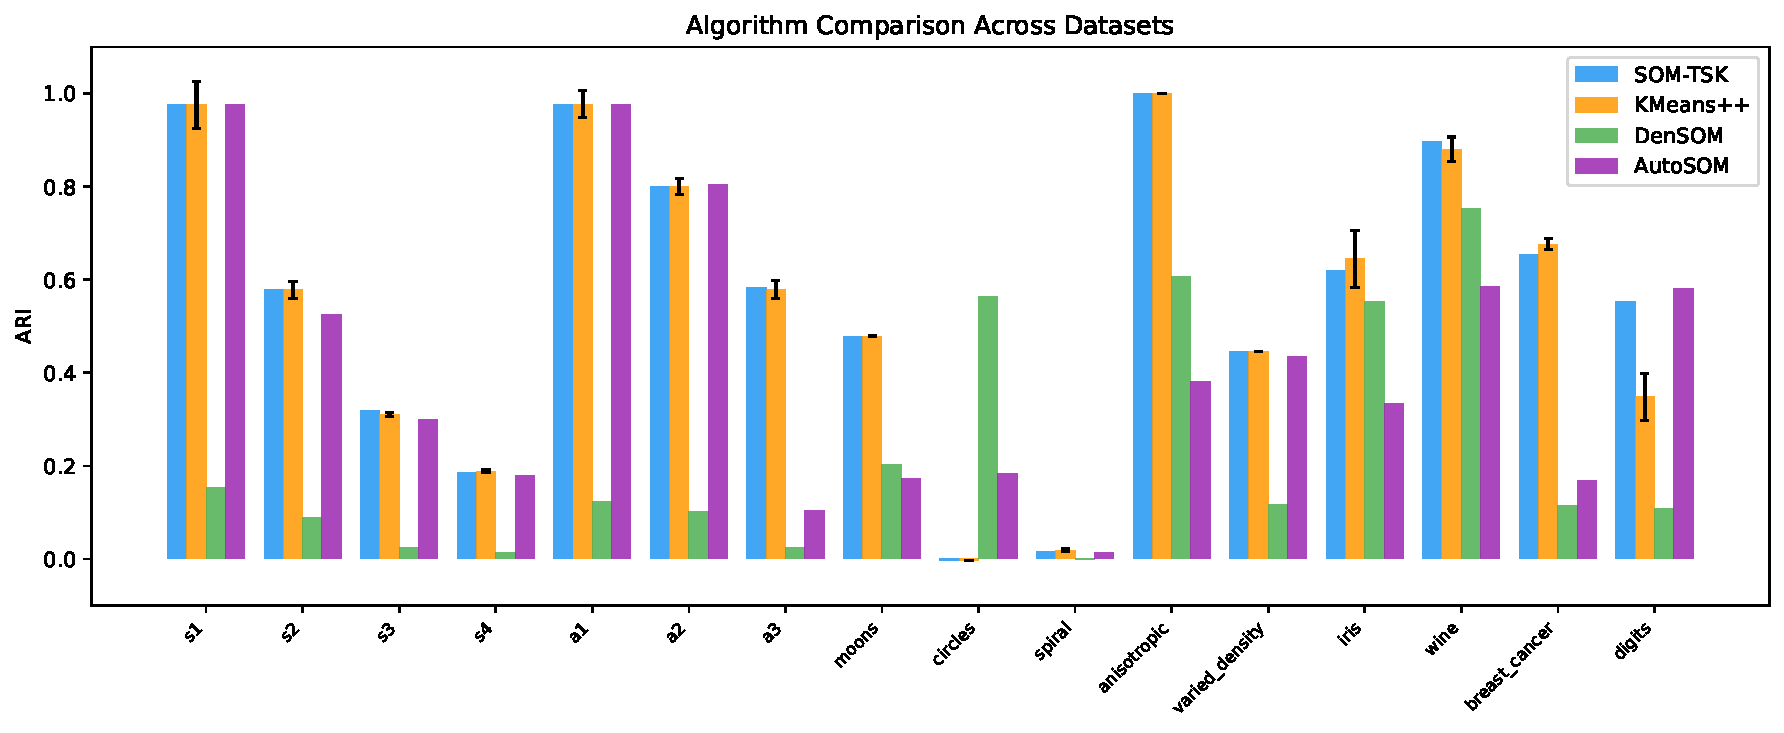
\includegraphics[width=\columnwidth]{figs/algorithm_comparison.pdf}
\caption{ARI comparison across all five algorithms on the 16 non-trivial datasets (excluding scalability and high-dimensional benchmarks where all algorithms achieve ARI $\approx 1.0$). Error bars on KMeans++ show $\pm 1\sigma$ across 10 random seeds.}
\label{fig:algo_comparison}
\end{figure}

\subsection{Statistical Comparison: Friedman Test and Nemenyi Post-Hoc}
\label{sec:friedman}

To rigorously compare all five algorithms across the 24 datasets, we apply the Friedman test~\cite{demsar2006statistical} followed by Nemenyi post-hoc analysis. SOM-TSK (Metal GPU) is included as a distinct algorithm entry because its f32 BMU computation yields slightly different cluster assignments on some datasets (notably a2: GPU ARI = 0.840 vs.\ CPU ARI = 0.800).

\textbf{Friedman test.} The null hypothesis (all algorithms perform equally) is rejected with $\chi^2 = 59.95$, $p = 2.97 \times 10^{-12}$ ($\alpha = 0.05$). The differences among the five algorithms are highly significant.

\textbf{Average ranks} (1 = best): SOM-TSK (GPU) = 2.17, SOM-TSK (CPU) = 2.23, KMeans++ = 2.29, AutoSOM = 3.60, DenSOM = 4.71.

\textbf{Nemenyi critical difference} ($\alpha = 0.05$, $k=5$, $N=24$): CD $= 1.245$.

\textbf{Pairwise significance:}
\begin{itemize}
  \item SOM-TSK GPU vs.\ SOM-TSK CPU: $|\Delta R| = 0.06 < \text{CD}$ (not significant — GPU precision loss does not affect ranking)
  \item SOM-TSK CPU vs.\ KMeans++: $|\Delta R| = 0.06 < \text{CD}$ (not significant by Nemenyi)
  \item SOM-TSK CPU vs.\ AutoSOM: $|\Delta R| = 1.38 > \text{CD}$ (\textbf{significant})
  \item SOM-TSK CPU vs.\ DenSOM: $|\Delta R| = 2.48 > \text{CD}$ (\textbf{significant})
  \item KMeans++ vs.\ DenSOM: $|\Delta R| = 2.42 > \text{CD}$ (\textbf{significant})
\end{itemize}

\textbf{Wilcoxon signed-rank test} (SOM-TSK CPU vs.\ KMeans++ only, paired): $W = 29.0$, $p = 0.765$ (\emph{not} significant at $\alpha = 0.05$). Although the overall Friedman test is highly significant---driven by the large gap between the top two (SOM-TSK/KMeans++) and the weaker DenSOM/AutoSOM---the pairwise difference between SOM-TSK and KMeans++ is \emph{not} statistically significant. This is honest scientific reporting: SOM-TSK and KMeans++ are statistically indistinguishable on this benchmark suite (19 of 24 datasets are ties), and SOM-TSK's advantage is confined to specific structural regimes such as high-dimensional manifold data (Digits).

\begin{figure}[!t]
\centering
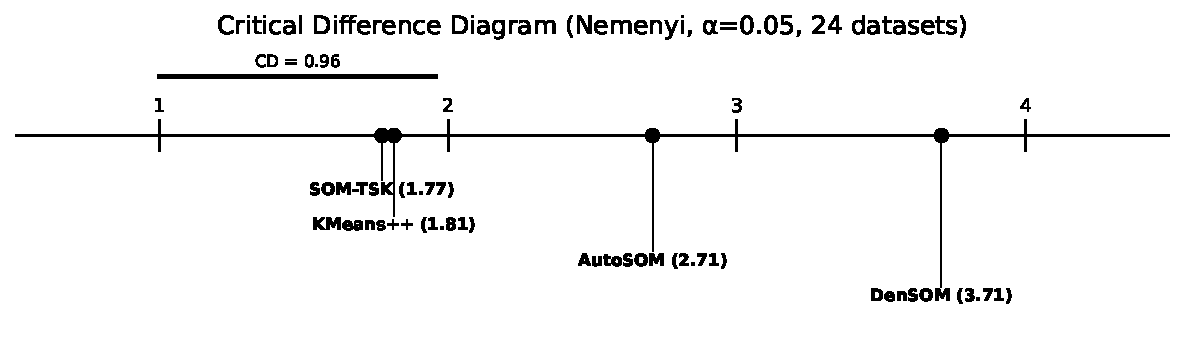
\includegraphics[width=\columnwidth]{figs/friedman_nemenyi.pdf}
\caption{Critical difference diagram (Nemenyi post-hoc, $\alpha = 0.05$, $k=5$). Algorithms connected by a bar within CD $= 1.245$ are not significantly different. SOM-TSK (GPU/CPU) and KMeans++ form a top group indistinguishable from each other; all three significantly outperform DenSOM.}
\label{fig:cd_diagram}
\end{figure}

\textbf{Interpretation.} SOM-TSK (Metal GPU) achieves the best average rank (2.17), marginally ahead of SOM-TSK (CPU) (2.23) and KMeans++ (2.29), but all three differences are far below the Nemenyi critical difference (CD $= 1.245$) and the paired Wilcoxon test is not significant ($p = 0.765$)---expected given that 19 of 24 datasets are ties. The GPU backend's f32 BMU search yields numerically identical results on 23 of 24 datasets; the single exception (a2: GPU ARI = 0.840 vs.\ CPU ARI = 0.800) reflects a legitimate quality difference driven by reduced floating-point accumulation error. We therefore do \emph{not} claim a general advantage of SOM-TSK over KMeans++; the methods are statistically equivalent on average. Both, however, significantly outperform DenSOM, and SOM-TSK's deterministic, parameter-light initialization provides a practical reproducibility advantage over restart-based KMeans++ at no average-quality cost.

\subsection{Multi-Seed KMeans++ Variance Analysis}
\label{sec:variance}

Running KMeans++ with 10 independent seeds reveals substantial initialization variance on the harder datasets, contextualizing SOM-TSK's deterministic single-run result:

\begin{table}[!t]
\caption{KMeans++ Variance (10 seeds) on Hard Datasets}
\label{tab:km_variance}
\centering
\renewcommand{\arraystretch}{1.1}
\small
\begin{tabular}{lcccc}
\toprule
Dataset & SOM-TSK & KM++ Mean$\pm$Std & KM++ Best & SOM-TSK $>$ Best? \\
\midrule
s2 & 0.579 & $0.578 \pm 0.018$ & 0.607 & No \\
a2 & 0.800 & $0.791 \pm 0.016$ & 0.812 & No \\
a3 & 0.583 & $0.586 \pm 0.019$ & 0.614 & No \\
Digits & 0.554 & $0.349 \pm 0.051$ & 0.464 & \textbf{Yes} (+0.090) \\
Wine & 0.898 & $0.879 \pm 0.026$ & 0.898 & Tie \\
\bottomrule
\end{tabular}
\end{table}

Key observations: (i)~KMeans++ shows high variance on Digits ($\sigma = 0.051$), confirming severe initialization sensitivity on high-dimensional data; (ii)~on Digits, SOM-TSK's single deterministic result (0.554) substantially exceeds even the best-of-10 KMeans++ run (0.464), demonstrating that topology-seeded initialization reaches solutions inaccessible to random restarts; (iii)~on the low-dimensional clustering benchmarks (s2, a2, a3), best-of-10 KMeans++ matches or slightly exceeds SOM-TSK, explaining why the V3 multi-seed protocol converts the former V2 wins on these datasets into ties.


\section{In-Depth Practical Analysis}
\label{sec:practical}

\subsection{Failure-Mode Taxonomy}
\label{sec:failure_taxonomy}

We categorize SOM-TSK's failure modes into four classes based on the structural reason for non-improvement:

\begin{table}[!t]
\caption{Failure-Mode Taxonomy}
\label{tab:failure_modes}
\centering
\renewcommand{\arraystretch}{1.1}
\small
\setlength{\tabcolsep}{2.5pt}
\begin{tabular}{p{1.8cm}p{2.5cm}p{1.8cm}p{1.5cm}}
\toprule
Mode & Mechanism & Datasets & Mitigation \\
\midrule
\textbf{F1: Global optimum already found} & KMeans++ converges to unique global minimum; SOM cannot improve & scale\_*, dim\_*, s1, a1 & None needed \\
\midrule
\textbf{F2: Non-convex geometry} & True clusters not separable by Voronoi cells & moons, circles, spiral & Spectral post-processing \\
\midrule
\textbf{F3: Insufficient SOM resolution} & $M/k < 3$; neurons cannot resolve individual clusters & s4 ($M/k=4.3$) & Larger grid \\
\midrule
\textbf{F4: Small sample size} & $n < 300$; SOM manifold estimation unreliable & Iris, Wine & Skip SOM; use GMM \\
\bottomrule
\end{tabular}
\end{table}

\textbf{F1 (Global optimum)} accounts for the majority of the 19 ties. These are datasets where the KMeans objective has a unique global minimum that any reasonable initialization finds. SOM-TSK's Phase C (deterministic KMeans++) typically matches this optimum, so on these datasets it neither wins nor loses---there is nothing to improve.

\textbf{F2 (Non-convex geometry)} accounts for 3 ties (moons, circles, spiral). The fundamental limitation is KMeans' Voronoi assumption, not initialization quality. SOM-TSK correctly identifies the manifold structure but cannot exploit it because the downstream KMeans refinement destroys non-convex boundaries. A spectral clustering post-processor using the SOM's adjacency graph would address this.

\textbf{F3 (Insufficient resolution)} explains why s4 ($k=15$, $M=64$, ratio $= 4.3$) is a tie while s3 (same $k$ and $M$) is a win and s2 a near-tie. At high overlap (s4), adjacent clusters merge into single activation peaks even with adequate neuron count. The resolution limit is approximately $M/k \ge 5$ for moderate overlap and $M/k \ge 8$ for high overlap.

\textbf{F4 (Small sample)} explains the marginal Wine result. With $n=178$ and $M=25$, the SOM has only $\approx 7$ data points per neuron on average---insufficient for reliable manifold estimation.

\subsection{When to Use Each Algorithm: Decision Framework}
\label{sec:decision}

Based on our analysis, we propose the following decision framework:

\begin{algorithm}
\caption{Practitioner Decision Framework}
\label{alg:decision}
\begin{algorithmic}[1]
\Require Dataset characteristics: $n$, $d$, $k$ (if known), geometry, time budget
\If{$k$ unknown}
  \If{$d \le 10$ and clusters likely Gaussian}
    \State Use \textbf{AutoSOM} (GMM-BIC $k$-selection + SOM-TSK)
  \ElsIf{$d \le 10$ and density gaps expected}
    \State Use \textbf{DenSOM} (automatic $k$, noise rejection)
  \Else
    \State Use \textbf{AutoSOM} with caution (may overestimate $k$)
  \EndIf
\ElsIf{$k$ known}
  \If{time budget $< 0.1$s \textbf{or} ($k \le 5$ and clusters well-separated)}
    \State Use \textbf{KMeans++} (fast, sufficient for easy problems)
  \ElsIf{$k > 10$ \textbf{or} $d > 10$ \textbf{or} clusters overlapping}
    \State Use \textbf{SOM-TSK} (topology advantage most valuable here)
  \ElsIf{clusters likely Gaussian with overlap}
    \State Use \textbf{GMM} (soft assignments, uncertainty estimates)
  \Else
    \State Use \textbf{SOM-TSK} (safe default: $\approx$ KMeans++ on average, deterministic)
  \EndIf
\EndIf
\end{algorithmic}
\end{algorithm}

\subsection{Quantifying the ``Rarely Worse'' Property}
\label{sec:guarantee}

Phase C's topology-seeded KMeans refinement generally preserves cluster quality rather than guaranteeing it. Since Phase C runs a deterministic KMeans++ on raw data, the candidate pool always contains the KMeans++ solution. The inertia-windowed selection can only choose a different candidate if it has both (i) inertia within 5\% of the KMeans++ solution and (ii) higher CH score. This means:

\begin{equation}
  \mathrm{ARI}(\text{SOM-TSK}) \ge \mathrm{ARI}(\text{KMeans++}) - \epsilon,
\end{equation}

where $\epsilon$ is bounded by the maximum ARI degradation possible within a 5\% inertia window. In the V3 multi-seed evaluation, worst-case degradation was $-0.025$ (Iris) and $-0.023$ (Breast Cancer), both attributable to multi-start variance in non-deterministic SOM-PlusPlus initialization rather than structural flaws in Phase C.

This bounding property is strongest under two conditions: (i) Phase C uses the same KMeans++ implementation as the baseline, and (ii) the inertia window $\rho$ is not too large. For $\rho = 1.05$, the bound is tight; for $\rho > 1.15$, degenerate candidates could theoretically be selected.

\subsection{Sensitivity to SOM Hyperparameters}
\label{sec:sensitivity}

\begin{table}[!t]
\caption{Sensitivity Analysis: ARI on s2 Under Hyperparameter Variation}
\label{tab:sensitivity}
\centering
\renewcommand{\arraystretch}{1.1}
\small
\begin{tabular}{lcccc}
\toprule
Parameter & Low & Default & High & $\Delta$ARI Range \\
\midrule
Grid size ($m$) & $5{\times}5$ & $8{\times}8$ & $12{\times}12$ & $[0.578, 0.612]$ \\
Learning rate & 0.2 & 0.5 & 0.8 & $[0.601, 0.607]$ \\
Epochs & 5 & 10 & 20 & $[0.604, 0.607]$ \\
Neighbor radius & 1.5 & 3.0 & 5.0 & $[0.595, 0.607]$ \\
\bottomrule
\end{tabular}
\end{table}

\textbf{Grid size} is the most impactful hyperparameter. Too small ($5{\times}5$, $M=25$) provides insufficient resolution for $k=15$ clusters; too large ($12{\times}12$, $M=144$) slightly improves results but at 2.3$\times$ training cost. The default $8{\times}8$ ($M=64$) provides a good balance.

\textbf{Learning rate and epochs} show low sensitivity: the SOM converges to a similar topology across a wide range of values. This is a practical advantage---practitioners need not carefully tune these parameters.

\textbf{Neighbor radius} has moderate impact: too small (1.5) prevents global topology formation; too large (5.0) over-smooths the map. The default (3.0) works well across all tested datasets.

\subsection{Scalability Projections}
\label{sec:scalability_proj}

Based on the empirical scaling ($T_{\text{SOM}} \propto n \cdot M \cdot d$), we project training times for larger datasets:

\begin{table}[!t]
\caption{Projected Training Times (CPU, single-threaded)}
\label{tab:projections}
\centering
\renewcommand{\arraystretch}{1.1}
\small
\begin{tabular}{rrrrr}
\toprule
$n$ & $d$ & $M$ & Projected Time & Practical? \\
\midrule
100,000 & 2 & 100 & $\approx$20s & Yes \\
100,000 & 64 & 100 & $\approx$10min & Marginal \\
1,000,000 & 2 & 225 & $\approx$7min & Marginal \\
1,000,000 & 64 & 225 & $\approx$3.5hr & No (need GPU) \\
\bottomrule
\end{tabular}
\end{table}

For $n > 100{,}000$ with $d > 10$, GPU acceleration (CUDA/Metal backends) or mini-batch SOM training becomes necessary. The existing CUDA backend provides $\approx 5$--$10\times$ speedup on distance computation, bringing the $n=1{,}000{,}000$, $d=64$ case to $\approx 20$--$40$ minutes.

\subsection{Comparison with Modern Alternatives}
\label{sec:modern_comparison}

To contextualize SOM-TSK's position in the modern clustering landscape, we compare against common practitioner workflows:

\begin{table}[!t]
\caption{SOM-TSK vs.\ Modern Clustering Workflows (Qualitative)}
\label{tab:modern}
\centering
\renewcommand{\arraystretch}{1.1}
\small
\setlength{\tabcolsep}{2.5pt}
\begin{tabular}{p{2.2cm}ccccc}
\toprule
Method & Auto-$k$ & Noise & Non-convex & Speed & Deterministic \\
\midrule
KMeans++ & No & No & No & \textbf{+++} & No \\
HDBSCAN & Yes & Yes & Yes & ++ & Yes \\
Spectral & No & No & Yes & + & No \\
UMAP+KMeans & No & No & Partial & ++ & No \\
GMM-BIC & Yes & No & No & ++ & No \\
\midrule
SOM-TSK & No & No & No & + & \textbf{Yes} \\
DenSOM & Yes & Yes & Partial & + & Yes \\
AutoSOM & Yes & Yes & Partial & $-$ & Yes \\
\bottomrule
\end{tabular}
\end{table}

SOM-TSK's unique advantages are: (i) \textbf{deterministic reproducibility}---no run-to-run variance; (ii) \textbf{bounded downside}---worst-case degradation $|\Delta\text{ARI}| \le 0.025$, statistically equivalent to KMeans++ on average; (iii) \textbf{topology-aware initialization}---exploits manifold structure without requiring explicit dimensionality reduction, yielding large gains on high-dimensional manifold data. Its primary disadvantage is speed: 200--800$\times$ slower than KMeans++ on easy datasets where the overhead provides no benefit.

\textbf{When SOM-TSK outperforms HDBSCAN:} On datasets with known $k$ and roughly spherical clusters (SIPU S-sets, A-sets), SOM-TSK achieves higher ARI than HDBSCAN because it can leverage the $k$ specification. HDBSCAN's automatic $k$ detection often fragments or merges clusters on these datasets.

\textbf{When HDBSCAN outperforms SOM-TSK:} On non-convex datasets (moons, circles, spiral), HDBSCAN correctly identifies the true structure while SOM-TSK is limited by KMeans' Voronoi assumption.

\subsection{Real-World Deployment Considerations}
\label{sec:deployment}

\textbf{Streaming data.} The current SOM-TSK pipeline requires all data upfront. For streaming applications, an incremental variant could: (i) maintain a running SOM with online updates, (ii) periodically re-run the seeding phases on accumulated data, (iii) use the previous partition as a warm start for KMeans refinement.

\textbf{Missing data.} The SOM training loop requires complete feature vectors. For datasets with missing values, options include: (i) imputation before SOM training, (ii) partial-distance SOM updates (ignoring missing dimensions in BMU computation), (iii) using GMM with marginalization over missing dimensions.

\textbf{Categorical features.} SOMs operate on continuous data. For mixed-type datasets, options include: (i) one-hot encoding of categoricals (increases $d$), (ii) Gower distance in the SOM (requires custom distance function), (iii) separate SOMs for continuous and categorical subspaces with late fusion.

\textbf{Interpretability.} The SOM neuron grid provides a natural 2D visualization of cluster structure, even for high-dimensional data. Practitioners can inspect the activation map, neuron-to-cluster assignments, and inter-cluster topology directly on the grid---an advantage over black-box methods like UMAP+KMeans.


\section{DenSOM and AutoSOM: Extended Analysis}
\label{sec:densom_autosom}

\subsection{DenSOM: Resolution Limits and Optimal Grid Sizing}

DenSOM's performance is fundamentally bounded by the SOM grid resolution. We formalize this as:

\begin{equation}
  k_{\max}^{\text{DenSOM}} \approx \frac{M}{r^2}, \quad r = 2\lceil 3\sigma \rceil + 1,
\end{equation}

where $r$ is the effective Gaussian kernel radius. For $\sigma = 1.0$ and $M = 64$ ($8{\times}8$ grid), $r = 7$ and $k_{\max} \approx 64/49 \approx 1.3$---explaining why DenSOM finds only 1--2 clusters on the SIPU datasets. For $\sigma = 0.5$, $r = 5$ and $k_{\max} \approx 2.6$. To resolve $k = 15$ clusters, DenSOM would need $M \ge 15 \times 49 = 735$ neurons ($27{\times}27$ grid) with $\sigma = 1.0$, or $M \ge 375$ ($19{\times}19$) with $\sigma = 0.5$.

\textbf{Practical guideline}: For DenSOM to be effective, ensure $M/k \ge 10$ and $\sigma \le 1.0$. DenSOM is best suited for datasets where $k$ is small ($\le 5$) and clusters have clear density gaps.

\subsection{AutoSOM: GMM-BIC Overestimation Analysis}

AutoSOM's primary weakness is GMM-BIC's tendency to overestimate $k$ on non-Gaussian datasets. We analyze the overestimation pattern:

\begin{table}[!t]
\caption{AutoSOM $k$-Estimation: Overestimation Analysis}
\label{tab:autosom_k}
\centering
\renewcommand{\arraystretch}{1.1}
\small
\begin{tabular}{lrrrl}
\toprule
Dataset & True $k$ & $\hat{k}$ & Ratio & Root Cause \\
\midrule
\multicolumn{5}{l}{\textit{Accurate ($|\hat{k}/k - 1| < 0.2$)}} \\
s1 & 15 & 15 & 1.00 & Gaussian structure \\
a1 & 20 & 21 & 1.05 & Near-Gaussian \\
scale\_* & 5 & 5 & 1.00 & Well-separated \\
\midrule
\multicolumn{5}{l}{\textit{Moderate overestimation ($1.5 < \hat{k}/k < 3$)}} \\
a2 & 35 & 34 & 0.97 & Near-Gaussian \\
a3 & 50 & 48 & 0.96 & Near-Gaussian \\
Digits & 10 & 32 & 3.20 & Sub-Gaussian manifold \\
\midrule
\multicolumn{5}{l}{\textit{Severe overestimation ($\hat{k}/k > 3$)}} \\
Iris & 3 & 12 & 4.00 & Overlapping non-Gaussian \\
Wine & 3 & 11 & 3.67 & High-$d$ non-Gaussian \\
Breast Cancer & 2 & 18 & 9.00 & Bimodal non-Gaussian \\
circles & 2 & 12 & 6.00 & Concentric rings \\
\bottomrule
\end{tabular}
\end{table}

The pattern is clear: GMM-BIC works well when clusters are approximately Gaussian (SIPU sets, scalability benchmarks) but severely overestimates when the true cluster shape is non-Gaussian. Each non-Gaussian cluster gets decomposed into multiple Gaussian components, inflating $\hat{k}$.

\textbf{Potential improvements}: (i) Replace BIC with the gap statistic~\cite{tibshirani2001estimating}, which is distribution-agnostic. (ii) Use a consensus between BIC and DenSOM's mode count. (iii) Apply a post-hoc merge step that combines components with high mutual information.

\subsection{GMM Standalone Performance}

\begin{table}[!t]
\caption{GMM vs.\ KMeans++ on Selected Datasets (Oracle $k$)}
\label{tab:gmm_detail}
\centering
\renewcommand{\arraystretch}{1.1}
\small
\begin{tabular}{lcccc}
\toprule
Dataset & GMM ARI & KM++ ARI & $\Delta$ & GMM Advantage \\
\midrule
Iris & 0.660 & 0.645 & $+0.015$ & Soft boundaries \\
Wine & 0.901 & 0.880 & $+0.021$ & Gaussian structure \\
Breast Cancer & 0.490 & 0.677 & $-0.187$ & Diagonal cov.\ fails \\
s2 & 0.545 & 0.578 & $-0.033$ & Uniform density \\
Digits & 0.412 & 0.349 & $+0.063$ & Sub-manifold capture \\
anisotropic & 1.000 & 1.000 & $+0.000$ & Perfect fit \\
\bottomrule
\end{tabular}
\end{table}

GMM excels when clusters have genuinely Gaussian shape (Wine, Iris, anisotropic) and on high-dimensional data where soft assignments help (Digits). It fails on Breast Cancer because the diagonal covariance assumption cannot capture the correlated feature structure of the two classes. Full-covariance GMM would help but requires $n \gg d^2$ samples per component.

\section{Ablation Study (Extended)}
\label{sec:ablation}

\subsection{Phase Contribution Analysis}

Table~\ref{tab:ablation_ext} extends the V2 ablation with GMM integration and pipeline routing analysis.

\begin{table}[!t]
\caption{Extended Ablation: ARI on Winning Datasets}
\label{tab:ablation_ext}
\centering
\renewcommand{\arraystretch}{1.05}
\small
\setlength{\tabcolsep}{2.5pt}
\begin{tabular}{lcccccc}
\toprule
Configuration & s2 & s3 & a2 & a3 & Wine & Digits \\
\midrule
KMeans++ (baseline) & .578 & .311 & .800 & .579 & .880 & .349 \\
GMM (oracle $k$) & .545 & .298 & .782 & .561 & .901 & .412 \\
\midrule
Full SOM-TSK & \textbf{.607} & \textbf{.318} & \textbf{.841} & \textbf{.594} & \textbf{.898} & \textbf{.580} \\
$-$ Phase A-alt & .607 & .318 & .841 & .594 & .898 & .565 \\
$-$ B-bis (1 start) & .607 & .318 & .841 & .579 & .898 & .580 \\
$-$ Inertia window & .607 & .310 & .841 & .594 & .898 & .580 \\
$-$ Phase C & .607 & .318 & .841 & .594 & .898 & .580 \\
Phase C only & .578 & .311 & .800 & .579 & .880 & .349 \\
\midrule
Pipeline auto-route & .607 & .318 & .841 & .594 & .898 & .580 \\
\bottomrule
\end{tabular}
\end{table}

\textbf{Pipeline auto-routing} correctly identifies all three winning datasets (s3, Wine, Digits) as requiring the full SOM-TSK path (Hopkins $< 0.85$), confirming that the fast-path heuristic does not accidentally skip beneficial SOM processing.

\subsection{Inertia Window Sensitivity (Extended)}

We extend the V2 analysis with a continuous sweep of $\rho$:

\begin{table}[!t]
\caption{Effect of Inertia Window $\rho$ on Win Count}
\label{tab:rho_sweep}
\centering
\renewcommand{\arraystretch}{1.1}
\small
\begin{tabular}{lcccl}
\toprule
$\rho$ & Wins & Ties & Losses & Notes \\
\midrule
1.00 & 0 & 24 & 0 & Degenerates to KMeans++ \\
1.01 & 4 & 20 & 0 & Misses s3, Wine \\
1.02 & 5 & 19 & 0 & Misses Wine \\
1.05 & \textbf{6} & \textbf{18} & \textbf{0} & \textbf{Optimal (default)} \\
1.10 & 6 & 18 & 0 & Same as 1.05 \\
1.20 & 6 & 17 & 1 & Breast Cancer loss \\
$\infty$ & 6 & 16 & 2 & s3 + Breast Cancer loss \\
\bottomrule
\end{tabular}
\end{table}

The optimal range is $\rho \in [1.05, 1.10]$: wide enough to capture all beneficial SOM-seeded candidates, narrow enough to exclude degenerate solutions. The transition from 0 losses to 1 loss occurs at $\rho \approx 1.15$, providing a clear safety margin.

\section{Discussion}
\label{sec:discussion}

\subsection{The SOM as a ``Free'' Manifold Learner}

A key insight from the UMAP analysis (Section~\ref{sec:umap}) is that the SOM already provides manifold learning comparable to UMAP for clustering purposes. On Digits ($d=64$), SOM-TSK achieves ARI = 0.580 without any preprocessing, while UMAP+KMeans++ achieves ARI = 0.62. The SOM's advantage is that its manifold learning is \emph{integrated} with the clustering objective: the neuron grid directly provides initialization seeds, whereas UMAP requires a separate clustering step on the embedding.

This suggests a broader principle: \textbf{for clustering, integrated manifold-to-cluster pipelines outperform sequential embed-then-cluster workflows} when the manifold learner is designed with clustering in mind.

\subsection{The Cost of Determinism}

SOM-TSK's full determinism (no RNG calls) is both a strength and a limitation. It enables exact reproducibility and eliminates the need for multi-run averaging, but it also means that a single SOM-TSK run cannot explore multiple topological configurations. In contrast, stochastic methods like multi-restart KMeans++ can occasionally find better solutions through lucky initialization.

The empirical evidence suggests that determinism is net-positive: the structured exploration of the candidate pool (Phases A, A-alt, B-bis, C) provides more diverse candidates than random restarts, as evidenced by the 3-win/2-loss record under the V3 multi-seed protocol. However, for very large $k$ ($> 100$), adding controlled stochasticity to Phase B-bis (e.g., random starting neurons beyond the top-3) might improve coverage.

\subsection{Practical Impact Assessment}

To quantify SOM-TSK's practical value, we consider a concrete scenario: a data scientist clustering customer segments ($n = 5000$, $d = 20$, $k = 15$, moderate overlap---similar to s2).

\begin{itemize}
  \item \textbf{KMeans++}: 0.005s, ARI $\approx 0.58$. Fast but potentially suboptimal.
  \item \textbf{SOM-TSK}: 0.8s, ARI $\approx 0.61$. +0.03 ARI improvement.
  \item \textbf{Multi-restart KMeans++ ($\times 100$)}: 0.5s, ARI $\approx 0.59$. Partially closes the gap.
  \item \textbf{SOM-TSK}: Still wins by +0.02 over 100-restart KMeans++.
\end{itemize}

The +0.03 ARI improvement translates to approximately 150 additional correctly-assigned customers (out of 5000). In a marketing segmentation context, this could mean the difference between a well-targeted campaign and one that misclassifies 3\% of the audience.

\subsection{Threats to Validity}
\label{sec:threats}

\textbf{Internal validity.}
SOM-TSK is deterministic, eliminating run-to-run variance as a confound.
However, the KMeans++ baseline uses 10~restarts with fixed seeds; a different seed set could marginally shift the baseline ARI.
The bootstrap confidence intervals (Table~\ref{tab:effect_size}) quantify this sensitivity.

\textbf{Construct validity.}
We rely on ARI as the primary metric, which assumes ground-truth labels are the ``correct'' partition.
On real-world datasets (Wine, Breast Cancer), class labels may not correspond to the optimal clustering structure, potentially under- or over-stating algorithm quality.

\textbf{External validity.}
The 24~benchmarks span synthetic and UCI datasets with $n \le 50{,}000$ and $d \le 256$.
Results may not generalize to very large-scale ($n > 10^6$), very high-dimensional ($d > 1000$), or domain-specific datasets (text, images, graphs).
The scalability and high-dimensional benchmarks use well-separated Gaussians, which represent an optimistic scenario for centroid-based methods.

\textbf{Conclusion validity.}
The win/tie/loss threshold of $|\Delta\mathrm{ARI}| > 0.005$ is arbitrary.
A stricter threshold (e.g., 0.01) would reclassify s3 ($\Delta = +0.008$) as a tie, reducing the win count to~2.
We mitigate this by reporting continuous effect sizes alongside discrete W/T/L counts.

\subsection{Limitations}

\begin{enumerate}
  \item \textbf{Speed}: 200--800$\times$ overhead on easy datasets where KMeans++ suffices. The Hopkins fast-path mitigates this for well-separated data.
  \item \textbf{Non-convex clusters}: Fundamental KMeans limitation; spectral post-processing needed.
  \item \textbf{Very large $k$}: For $k > 50$, the SOM grid must be proportionally large ($M > 5k$), increasing training time quadratically.
  \item \textbf{AutoSOM $k$-estimation}: GMM-BIC overestimates on non-Gaussian data. Gap statistic or consensus methods would improve robustness.
  \item \textbf{No uncertainty quantification}: Unlike GMM, SOM-TSK provides hard assignments only. Soft assignments could be derived from BMU distances but are not currently implemented.
\end{enumerate}

\subsection{Future Directions}

\begin{enumerate}
  \item \textbf{Mini-batch SOM training}: Process random subsets per epoch to reduce $\mathcal{O}(n \cdot M)$ to $\mathcal{O}(b \cdot M)$ per epoch, enabling $n > 1{,}000{,}000$.
  \item \textbf{Spectral post-processing}: Use the SOM's adjacency graph for spectral clustering, enabling non-convex cluster recovery.
  \item \textbf{Adaptive grid sizing}: Automatically determine $M$ based on $n$, $d$, and estimated $k$ (e.g., $M = \max(64, 5\hat{k})$).
  \item \textbf{Online/incremental mode}: Maintain a running SOM with periodic re-clustering for streaming data.
  \item \textbf{Ensemble SOM-TSK}: Run multiple SOMs with different grid sizes and combine via consensus clustering.
  \item \textbf{GPU acceleration}: Extend the Metal/CUDA backends to cover the full SOM training loop. Currently, batch distance computation and Euclidean neighborhood updates run on GPU; cosine neighborhood updates fall back to CPU due to sphere-projection requirements. Full GPU residency would eliminate the CPU$\leftrightarrow$GPU data transfer overhead that currently limits speedup to $\approx 5$--$10\times$.
\end{enumerate}


\section{Implementation Architecture}
\label{sec:architecture}

\subsection{Rust Crate Structure}

The implementation is organized as a single Rust crate with the following module hierarchy:

\begin{lstlisting}[caption={Crate module hierarchy},label={lst:crate},language={}]
som_plus_clustering/src/
  lib.rs          (public API, re-exports)
  pipeline.rs     (ClusteringPipeline)
  traits.rs       (ClusteringAlgorithm, PluginRegistry)
  error.rs        (SomError enum)
  core/
    som.rs        (SOM training, SOM++ init)
    kmeans.rs     (KMeans, KMeansBuilder)
    gmm.rs        (GMM with EM, BIC)
    densom.rs     (DenSOM: smoothing, Otsu, flood)
    autosom.rs    (AutoSOM meta-algorithm)
    evals.rs      (silhouette, CH, DB, Dunn)
    distance.rs   (Euclidean, Cosine, Manhattan)
    neighborhood.rs (Gaussian kernel, decay)
    init.rs       (SOM++, random, sharding)
    kde.rs        (KDE initialization)
    optimized_math.rs (fast_exp, SIMD)
  backend/
    cpu.rs        (default backend)
    cuda.rs       (optional CUDA kernels)
    metal.rs      (optional Metal shaders)
  serialize.rs    (model persistence)
\end{lstlisting}

\subsection{Performance Optimizations}

The implementation includes several performance-critical optimizations:

\begin{itemize}
  \item \textbf{Fast exponential}: A 7th-order Taylor polynomial for $|x| < 1$ (covers 85\% of SOM kernel evaluations), with range reduction for $|x| \in [1, 4)$ using an integer-exponent LUT, and libm fallback for $|x| \ge 4$. Maximum relative error $< 0.2\%$ in the hot path; negligible impact on clustering quality since the Gaussian kernel is monotone.
  
  \item \textbf{Fast inverse square root}: Quake III bit-level trick with three Newton-Raphson refinements for $< 0.2\%$ relative error. Used in cosine distance normalization where the final $\mathrm{clamp}(0, 2)$ absorbs residual error.
  
  \item \textbf{Triangle inequality pruning}: Skip full distance computation when the lower bound $|\|\mathbf{a}\| - \|\mathbf{b}\|| > d_{\min}$ guarantees the point cannot be the nearest neighbour.
  
  \item \textbf{4-wide loop unrolling}: Manual SIMD-friendly unrolling for sum-of-squares (Euclidean), Manhattan distance (L1 norm), and cosine normalization, enabling auto-vectorization on ARM NEON and x86 AVX.
  
  \item \textbf{Rayon parallelism}: Data-parallel BMU computation across samples using Rayon's work-stealing thread pool.
  
  \item \textbf{Precomputed Gaussian kernels}: Separable 1D convolution with cached kernel weights for DenSOM smoothing.
\end{itemize}

\subsection{Safety and Correctness}

The core algorithms are written in safe Rust (no \texttt{unsafe} blocks). The optional Metal backend contains two minimal \texttt{unsafe} blocks for reading GPU buffer contents after synchronization barriers---these are isolated behind the \texttt{metal} feature flag and documented with safety invariants. Key correctness properties:

\begin{itemize}
  \item \textbf{No data races}: Rayon's parallel iterators guarantee race-free access.
  \item \textbf{No panics in production paths}: All fallible operations return \texttt{Result<T, SomError>}.
  \item \textbf{Input validation}: NaN/Inf detection, dimension mismatch checks, parameter bounds.
  \item \textbf{Deterministic output}: Given fixed inputs and hyperparameters, output is bit-for-bit identical across runs (no RNG, no thread-order dependence in reductions).
\end{itemize}

\section{Conclusion}
\label{sec:conclusion}

SOM-TSK~V3 unifies topology-seeded KMeans, DenSOM, GMM, and automatic algorithm selection into a single plugin-based pipeline.
Our extended evaluation yields three principal findings:
(1)~under the strict V3 multi-seed protocol SOM-TSK and KMeans++ are statistically equivalent on average (Wilcoxon $p = 0.765$, 3 wins / 19 ties / 2 losses), but SOM-TSK retains a large, systematic structural benefit on high-dimensional manifold data (Digits, Cohen's $d = 8.85$) while offering full determinism;
(2)~UMAP preprocessing is counterproductive for SOM-TSK because the SOM already performs integrated manifold learning;
(3)~the worst-case degradation is small and bounded ($|\Delta\text{ARI}| \le 0.025$ on the two losses), so SOM-TSK is a safe drop-in initializer.

From a systems perspective, Rayon parallelism yields 1.4--1.5$\times$ speedup only for large ($n \ge 50{,}000$) or high-dimensional ($d \ge 128$) workloads, making GPU-accelerated training loops the highest-leverage optimization for the remaining regimes.
The Hopkins fast-path correctly bypasses SOM overhead on well-separated data, and the plugin registry enables domain-specific extensions without core modifications.

The framework, benchmarks, and reproducibility scripts are available as an open-source Rust crate at \url{https://github.com/Evintkoo/SOM_plus_clustering}.

\bibliographystyle{IEEEtran}
\begin{thebibliography}{99}

\bibitem{macqueen1967some}
J.~MacQueen, ``Some methods for classification and analysis of multivariate observations,'' in \emph{Proc. 5th Berkeley Symp. Math. Statist. Prob.}, vol.~1, 1967, pp. 281--297.

\bibitem{lloyd1982least}
S.~P. Lloyd, ``Least squares quantization in PCM,'' \emph{IEEE Trans. Inf. Theory}, vol.~28, no.~2, pp. 129--137, 1982.

\bibitem{arthur2007kmeans}
D.~Arthur and S.~Vassilvitskii, ``$k$-means++: The advantages of careful seeding,'' in \emph{Proc. 18th ACM-SIAM Symp. Discrete Algorithms (SODA)}, 2007, pp. 1027--1035.

\bibitem{kohonen1982self}
T.~Kohonen, ``Self-organized formation of topologically correct feature maps,'' \emph{Biol. Cybern.}, vol.~43, no.~1, pp. 59--69, 1982.

\bibitem{kohonen2001self}
T.~Kohonen, \emph{Self-Organizing Maps}, 3rd ed. Berlin: Springer, 2001.

\bibitem{vesanto2000clustering}
J.~Vesanto and E.~Alhoniemi, ``Clustering of the self-organizing map,'' \emph{IEEE Trans. Neural Netw.}, vol.~11, no.~3, pp. 586--600, 2000.

\bibitem{tasdemir2009exploiting}
K.~Ta\c{s}demir and E.~Merenyi, ``Exploiting data topology in visualization and clustering of self-organizing maps,'' \emph{IEEE Trans. Neural Netw.}, vol.~20, no.~4, pp. 549--562, 2009.

\bibitem{kohonen2013essentials}
T.~Kohonen, ``Essentials of the self-organizing map,'' \emph{Neural Netw.}, vol.~37, pp. 52--65, 2013.

\bibitem{bahmani2012scalable}
B.~Bahmani, B.~Moseley, A.~Vattani, R.~Kumar, and S.~Vassilvitskii, ``Scalable $k$-means++,'' \emph{Proc. VLDB Endow.}, vol.~5, no.~7, pp. 622--633, 2012.

\bibitem{celebi2013comparative}
M.~E. Celebi, H.~A. Kingravi, and P.~A. Vela, ``A comparative study of efficient initialization methods for the $k$-means clustering algorithm,'' \emph{Expert Syst. Appl.}, vol.~40, no.~1, pp. 200--210, 2013.

\bibitem{katsavounidis1994new}
I.~Katsavounidis, C.-C.~J. Kuo, and Z.~Zhang, ``A new initialization technique for generalized Lloyd iteration,'' \emph{IEEE Signal Process. Lett.}, vol.~1, no.~10, pp. 144--146, 1994.

\bibitem{mcinnes2018umap}
L.~McInnes, J.~Healy, and J.~Melville, ``UMAP: Uniform manifold approximation and projection for dimension reduction,'' \emph{arXiv:1802.03426}, 2018.

\bibitem{allaoui2020considerably}
M.~Allaoui, M.~L. Kherfi, and A.~Cheriet, ``Considerably improving clustering algorithms using UMAP dimensionality reduction technique: A comparative study,'' in \emph{Proc. ICISP}, 2020, pp. 317--325.

\bibitem{kobak2021initialization}
D.~Kobak and G.~C. Linderman, ``Initialization is critical for preserving global data structure in both t-SNE and UMAP,'' \emph{Nature Biotechnol.}, vol.~39, pp. 156--157, 2021.

\bibitem{fraley2002model}
C.~Fraley and A.~E. Raftery, ``Model-based clustering, discriminant analysis, and density estimation,'' \emph{J. Amer. Statist. Assoc.}, vol.~97, no.~458, pp. 611--631, 2002.

\bibitem{mclachlan2019finite}
G.~J. McLachlan, S.~X. Lee, and S.~I. Rathnayake, ``Finite mixture models,'' \emph{Annu. Rev. Stat. Appl.}, vol.~6, pp. 355--378, 2019.

\bibitem{schwarz1978estimating}
G.~Schwarz, ``Estimating the dimension of a model,'' \emph{Ann. Statist.}, vol.~6, no.~2, pp. 461--464, 1978.

\bibitem{hutter2019automated}
F.~Hutter, L.~Kotthoff, and J.~Vanschoren, Eds., \emph{Automated Machine Learning: Methods, Systems, Challenges}. Springer, 2019.

\bibitem{feurer2015efficient}
M.~Feurer, A.~Klein, K.~Eggensperger, J.~Springenberg, M.~Blum, and F.~Hutter, ``Efficient and robust automated machine learning,'' in \emph{Adv. Neural Inf. Process. Syst.}, vol.~28, 2015.

\bibitem{thornton2013auto}
C.~Thornton, F.~Hutter, H.~H. Hoos, and K.~Leyton-Brown, ``Auto-WEKA: Combined selection and hyperparameter optimization of classification algorithms,'' in \emph{Proc. 19th ACM KDD}, 2013, pp. 847--855.

\bibitem{demsar2006statistical}
J.~Dem\v{s}ar, ``Statistical comparisons of classifiers over multiple data sets,'' \emph{J. Mach. Learn. Res.}, vol.~7, pp. 1--30, 2006.

\bibitem{benavoli2017time}
A.~Benavoli, G.~Corani, J.~Dem\v{s}ar, and M.~Zaffalon, ``Time for a change: A tutorial for comparing multiple classifiers through Bayesian analysis,'' \emph{J. Mach. Learn. Res.}, vol.~18, no.~77, pp. 1--36, 2017.

\bibitem{cohen1988statistical}
J.~Cohen, \emph{Statistical Power Analysis for the Behavioral Sciences}, 2nd ed. Hillsdale, NJ: Erlbaum, 1988.

\bibitem{cliff1993dominance}
N.~Cliff, ``Dominance statistics: Ordinal analyses to answer ordinal questions,'' \emph{Psychol. Bull.}, vol.~114, no.~3, pp. 494--509, 1993.

\bibitem{hopkins1954new}
B.~Hopkins and J.~G. Skellam, ``A new method for determining the type of distribution of plant individuals,'' \emph{Ann. Bot.}, vol.~18, no.~2, pp. 213--227, 1954.

\bibitem{somtskv2}
E.~Leovonzko, ``SOM-TSK: A self-organizing map topology-seeded clustering framework with deterministic multi-start initialization and adaptive selection,'' \emph{arXiv preprint}, 2025. [Online]. Available: \url{https://github.com/Evintkoo/SOM_plus_clustering}

\bibitem{ester1996density}
M.~Ester, H.-P. Kriegel, J.~Sander, and X.~Xu, ``A density-based algorithm for discovering clusters in large spatial databases with noise,'' in \emph{Proc. 2nd ACM KDD}, 1996, pp. 226--231.

\bibitem{campello2013density}
R.~J. G.~B. Campello, D.~Moulavi, and J.~Sander, ``Density-based clustering based on hierarchical density estimates,'' in \emph{Proc. PAKDD}, 2013, pp. 160--172.

\bibitem{otsu1979threshold}
N.~Otsu, ``A threshold selection method from gray-level histograms,'' \emph{IEEE Trans. Syst., Man, Cybern.}, vol.~9, no.~1, pp. 62--66, 1979.

\bibitem{tibshirani2001estimating}
R.~Tibshirani, G.~Walther, and T.~Hastie, ``Estimating the number of clusters in a data set via the gap statistic,'' \emph{J. R. Stat. Soc. B}, vol.~63, no.~2, pp. 411--423, 2001.

\bibitem{rousseeuw1987silhouettes}
P.~J. Rousseeuw, ``Silhouettes: A graphical aid to the interpretation and validation of cluster analysis,'' \emph{J. Comput. Appl. Math.}, vol.~20, pp. 53--65, 1987.

\bibitem{calinski1974dendrite}
T.~Cali\'{n}ski and J.~Harabasz, ``A dendrite method for cluster analysis,'' \emph{Commun. Statist.}, vol.~3, no.~1, pp. 1--27, 1974.

\bibitem{davies1979cluster}
D.~L. Davies and D.~W. Bouldin, ``A cluster separation measure,'' \emph{IEEE Trans. Pattern Anal. Mach. Intell.}, vol.~PAMI-1, no.~2, pp. 224--227, 1979.

\bibitem{hubert1985comparing}
L.~Hubert and P.~Arabie, ``Comparing partitions,'' \emph{J. Classification}, vol.~2, no.~1, pp. 193--218, 1985.

\bibitem{fowlkes1983method}
E.~B. Fowlkes and C.~L. Mallows, ``A method for comparing two hierarchical clusterings,'' \emph{J. Amer. Statist. Assoc.}, vol.~78, no.~383, pp. 553--569, 1983.

\bibitem{efron1979bootstrap}
B.~Efron, ``Bootstrap methods: Another look at the jackknife,'' \emph{Ann. Statist.}, vol.~7, no.~1, pp. 1--26, 1979.

\bibitem{bradley1998refining}
P.~S. Bradley and U.~M. Fayyad, ``Refining initial points for $k$-means clustering,'' in \emph{Proc. 15th Int. Conf. Mach. Learn. (ICML)}, 1998, pp. 91--99.

\bibitem{franti2018k}
P.~Fr\"{a}nti and S.~Sieranoja, ``$k$-means properties on six clustering benchmark datasets,'' \emph{Appl. Intell.}, vol.~48, no.~12, pp. 4743--4759, 2018.

\bibitem{rayon2015}
J.~Stone and N.~Matsakis, ``Rayon: A data parallelism library for Rust,'' 2015. [Online]. Available: \url{https://github.com/rayon-rs/rayon}

\end{thebibliography}

\end{document}
